\section{Introduction}
The paraphrase of a sentence retains its meaning but makes different choices
of words and expressions than the original form. 
Paraphrase generation plays an important role in many downstream tasks, 
such as question answering, machine translation, and information 
retrieval~\cite{hu2019improved}. 
% \KZ{In this para, you should define
% what are supervised, unsupervised, weakly supervised paraphrasing
% tasks, etc. And be very clear what is the nature of our task in this paper.}

% Domain adaptation is a common requirement in supervised paraphrase generation 
% since 
Most existing parallel datasets for paraphrase generation are 
domain-specific. Quora and WikiAnswers \cite{fader2013paraphrase} datasets 
only contain questions; sentences in MSCOCO \cite{lin2014microsoft} dataset 
are mostly descriptions for physical objects since they are the captions of 
images; 
and PPDB \cite{ganitkevitch2013ppdb} contains phrases rather than sentences. 
The performance of a model trained with these domain-specific parallel data 
declines seriously when it is used in another domain \cite{li2019decomposable}. 
% \KZ{But you just said
% domain adaptation is a common requirement. Does that fix the problem or not?
% You left me wondering..} 
% Therefore, unsupervised and distance-supervised methods
% are often used for paraphrase generation.

Many efforts were made to solve this domain adaptation problem. These efforts are roughly divided into three directions: unsupervised fine-tuning for supervised model, unsupervised methods based on word/phrase replacement, and distantly-supervised methods based on bilingual data.
% \KZ{Don't use refs as subjects or objects of a setence! Use author plus shortcite or citeauthor instead. Check this throughout the paper.} 
\citeauthor{li2019decomposable}~\shortcite{li2019decomposable} chose to fine-tune the supervised model with non-parallel in-domain data, but the performance of their model decreases a lot when the domain span is large.
\citeauthor{liu2019unsupervised}~\shortcite{liu2019unsupervised} and \citeauthor{miao2019cgmh}~\shortcite{miao2019cgmh} used unsupervised methods to generate paraphrases, but their models are mostly based on the variation of 
words and phrases and can hardly change the structure of the whole sentence. 
\citeauthor{wieting2017paranmt}~\shortcite{wieting2017paranmt} generated paraphrases with a round-trip translation model, but the existing translation models are sometimes not very accurate, which also affects the performance of their method. \citeauthor{liu2020exploring}~\shortcite{liu2020exploring} use bilingual data to train an unsupervised model, but their improvement is mainly brought about by the follow-up supervised fine-tuning.
% \KZ{you sound like unsupervised
% methods should achieve better than unsupervised methods. But in your
% results, your results only match supervised methods with DA in some of
% the datasets. This seems to suggest that unsupervised methods are not
% as strong as supervised. Seems to contradict.}

% \KZ{What are the common approaches in previous unsupervised methods? What 
% are the disadvantages? Did they not capture the human intuition when
% doing paraphrase?}
% 
% \KZ{The following is only one possible human paraphrase process.
% It is unconfirmed so say it with care. Instead of ``hidden meaning'',
% maybe say ``underlying semantics''.}

% Existing unsupervised methods are mostly based on the variation of 
% words and phrases and can hardly change the structure of the whole sentence. 
% For example, \cite{liu2019unsupervised} proposed a method using simulated 
% annealing for words and phrases, and \cite{miao2019cgmh} used Metropolis Hastings in the word space. 

% Inspired by Denoising Auto-Encoder(DAE, \cite{denoisingAE}) and back-translation, 
In this paper, we propose a novel paraphrase generation framework that does not require any parallel paraphrase data and can be applied in any domain. 
\footnote{Code is available: \url{https://codeocean.com/capsule/6125185/tree/v1}}
In our framework, two kinds of underlying semantics are extracted from 
the original sentence and are recombined into a new sentence through 
a hybrid decoder.

% In this paper, we propose a novel unsupervised paraphrase generation 
% framework that can alter the expression at the sentence level. 
% We extract the underlying semantics from the original sentence and 
% extend it into a new sentence. Information loss may occur when 
% extracting semantics. To retain more information of the original sentence, 
% we extract in two different directions and combine the extracted 
% information in a hybrid decoder 
% % (\secref{sec:joint}) 
% to generate paraphrases.

The first kind of underlying semantics is represented by a word set, 
which is inspired by the Denoising Auto-Encoder (DAE)~\cite{denoisingAE}. 
A bag of words is a great carrier of information, 
as it communicates the central idea without syntactic constraints. 
People can produce different sentences with similar meaning from the same 
set of words. Table~\ref{para-example} shows an example of such 
paraphrase sentences. We construct a word set from the 
original sentence and extend the word set into a complete sentence 
with a set-to-sequence (set2seq) model, % (\secref{sec:set2seq})
which is adapted from the well-known sequence-to-sequence (seq2seq) model 
by ignoring the sequential information from the input sequence.

\begin{table}[th]
\small
\centering
\begin{tabular}{l}
\hline 
word set: \textbf{(man, sit, bike, bench)} \\
\hline
A \textit{\color{red}man} is \textit{\color{red}sitting} on a \textit{\color{red}bench} next to a \textit{\color{red}bike} \\
A \textit{\color{red}man} is \textit{\color{red}sitting} on a \textit{\color{red}bench} next to a \textit{\color{red}bicycle} \\
A \textit{\color{red}man sits} on a \textit{\color{red}bench} by a \textit{\color{red}bike} \\
\textit{\color{red}Man sitting} on a \textit{\color{red}bench} near a personal \textit{\color{red}bicycle} \\
A \textit{\color{red}man} is \textit{\color{red}sitting} on a \textit{\color{red}bench} with a \textit{\color{red}bike} \\
\hline
\end{tabular}
\caption{\label{para-example} Paraphrases formed
from a word set.} 
\end{table}


% \KZ{Don't have to say Chinese specifically here. Can be any language.}
The second carrier of semantics is the translation of the 
original sentence into another language. 
Semantics is preserved but syntactic perturbations are added 
when the translation is then translated back to the 
original language. This is known as round-trip translation~\cite{wieting2017paranmt}. 

% \footnote{Considering that training the back-translation model requires 
% intensive computing resources, we will open-source these models and the codes
% when the paper is published.}
% \KZ{In previous backtranslation methods, do they assume that the model is
% a white box and the code can be used? If not, I think we need to say it clear
% here that what assumptions we are making: we have access to a trained 
% translation model as well as its code during the decoding phase. Otherwise
% the readers may complain that we are going them false hope.}  

\begin{figure*}[h]
\centering
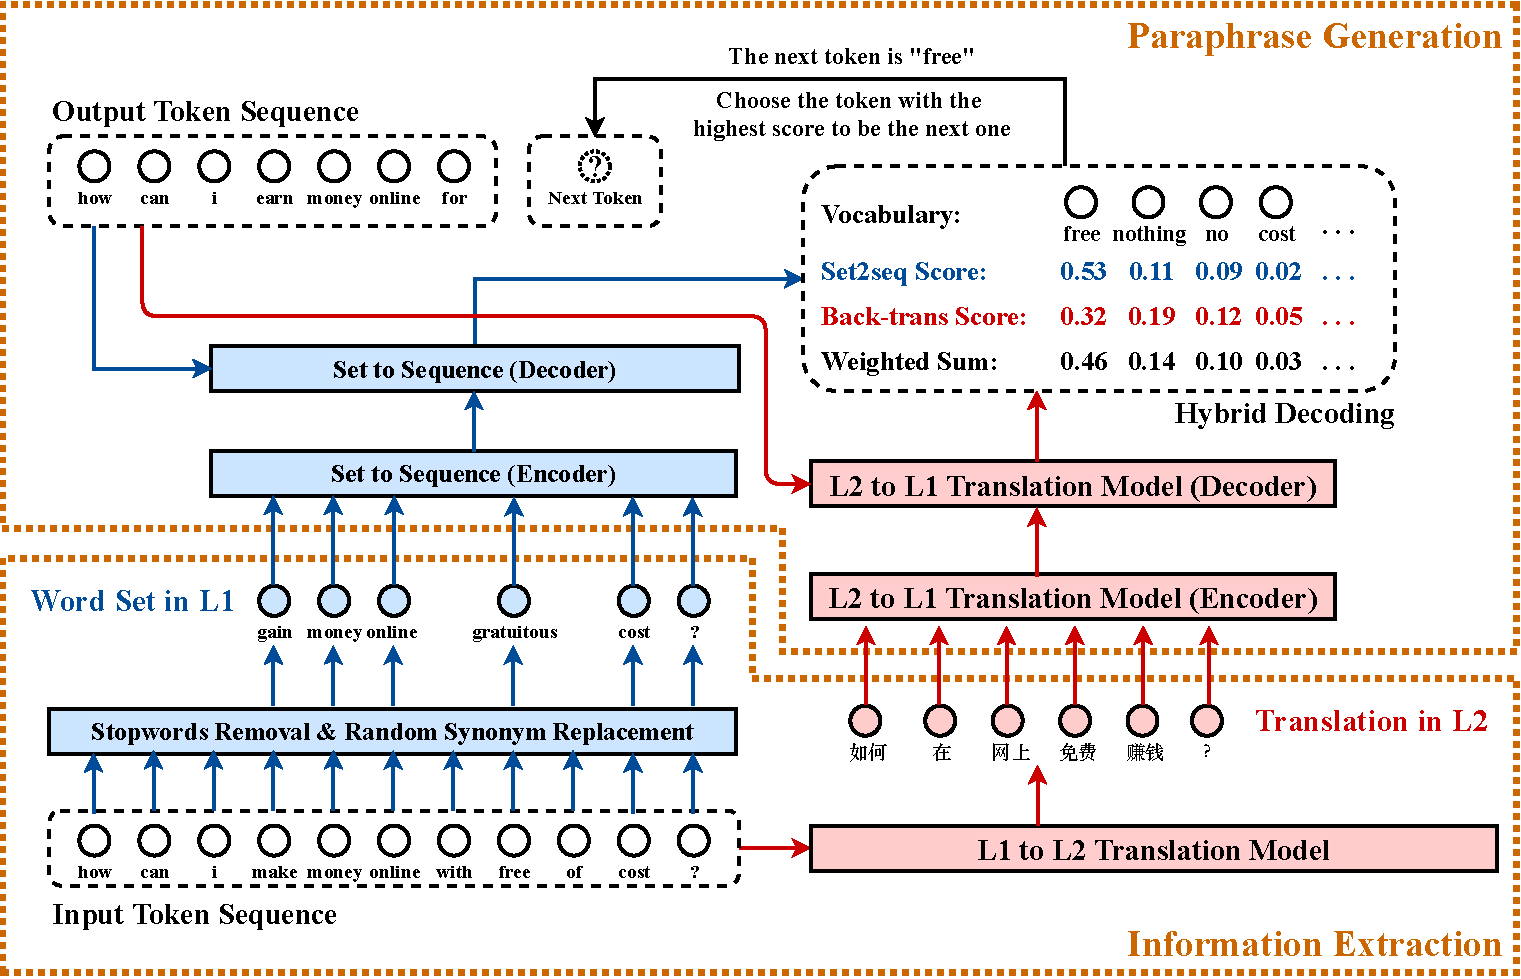
\includegraphics[width=1.6\columnwidth]{Paraphrase.pdf}
\caption{Our Paraphrasing Framework}
\label{fig:app}
\end{figure*}
 
The above two types of semantics are complementary. The round-trip translation makes 
up for the missing information in the set2seq model, such as sequential information. The set2seq model gives the round-trip translation model some lexical hints 
and makes the translation result more accurate. We thus integrate the decoding parts of 
the set2seq model and the round-trip translation model to jointly generate paraphrases.

We evaluate our framework on four paraphrasing datasets, namely Quora, WikiAnswers, MSCOCO, and Twitter \cite{lan2017continuously}, and achieve the state-of-the-art accuracies compared to existing models trained with non-parallel data. 
% For supervised models with unsupervised domain-adaptation 
% , we only compare our method with them in Quora and WikiAnswers since the results of the SOTA method~\cite{li2019decomposable} are only 
%available on Quora and WikiAnswers.

% \KZ{This para sounds a bit repeat from paragraph 1. The connection is
% a bit strange. Consider restructuring it.}
% Domain-adaptation is to train the model with parallel paraphrasing pairs 
% in the source domain and fine-tune the model with non-parallel sentences 
% in the target domain, which can also be considered unsupervised from 
% the perspective of the target domain. Therefore, we also compare 
% our method with domain-adaptation supervised methods with  in 
% Quora and WikiAnswers. The comparison is not on all four datasets 
% because results of the SOTA method~\cite{li2019decomposable} are only 
% available on Quora and WikiAnswers.

% \KZ{Instead of cross-domain, call it ``common-domain'' or ``general-domain'',
% to go inline with the name of this model?}
We also train the set2seq model on a big common-domain dataset and test it on these four datasets, and still obtain decent results. We call the set2seq model trained from the big common-domain dataset ``set2seq-common'', and can
apply it to any domain when there is no in-domain data to train a set2seq model.

% Both unsupervised methods and supervised methods with domain-adaptation require the non-parallel data from the target domain. However, there is not 
% always enough data for training. For example, the Twitter dataset only has 
% 110K non-parallel training data. To this end, we trained the set2seq model on a big cross-domain dataset, name it ``set2seq-common''. We use the set2seq-common instead of the domain-specific set2seq models on four datasets, and still receive decent results.

Finally, we propose an application of our paraphrase generator: 
to augment the training data of 
a neural machine translation (NMT) model between low-resource languages 
and English. 
We paraphrase the English sentences in the parallel training pairs 
with set2seq-common and improve the BLEU score of X-to-English 
translation by 1.53 to 2.17, where X is a low-resource language.

In summary, the main contributions of this work are:
\begin{itemize}
\item We are the first to apply the set2seq model to the task of paraphrase generation by combining it with a round-trip translation model through a hybrid decoder.
%\item We are the first to combine the set2seq model with the back-translation model through a hybrid decoder. \KZ{A bit strange: why do we need to 
%combine the two? Maybe say this is a novel architecture.}
\item The framework proposed by us achieve state-of-the-art accuracies on 
four benchmark datasets compared with existing methods.
\item We apply our method to augment the training data of low-resource
translation tasks and obtain significant improvement in translation quality.
\end{itemize}
